\documentclass[colophon]{phduio}

\usepackage{phdstyle}   % Custom style
\usepackage{kantlipsum} % Dummy text

\author{Author}
\title{Working Title}
\department{Department}
\faculty{Faculty}
\affiliation
{
    Optional Second Affiliation
    \and
    Optional Further Specification
}
\ISSN{1234-5678}
\dissertationseries{1234}


\includeonly
{
    sections/dedication,
    sections/abstract,
    sections/preface,
    sections/introduction,
    sections/chapter2,
    sections/chapter3,
    sections/chapter4,
    sections/appendixA,
    sections/appendixB,
}

\begin{document}

    \frontmatter        % Folios in Roman numerals, unnumbered chapters.

    \uiotitle

    \thispagestyle{empty}
\vspace*{\stretch{1}}
\begin{flushright}
    \emph{To my ghostwriter}
\end{flushright}
\vspace*{\stretch{3}}
    \chapter{Abstract}
\kant[1-3] % Dummy text
\todo[inline]{Add new section about results in \cref{sec:fourth}.}

% OPTIONAL SOLUTION:

% Use these settings if you are writing a monograph
% and have only one abstract.
% Do not use them if you have an abstract
% at the beginning of each chapter/paper.

% \abstractintoc % Add abstract to Table of Contents
% \abstractnum   % Format abstract like a chapter

%\begin{abstract}
%    \kant[1-3] % Dummy text
%    \todo[inline]{Add new section about results in \cref{sec:fourth}.}
%\end{abstract}
    \chapter{Preface}


This is where you write your personal experiences with the thesis, making a note of collaborations and contributions to authorship.

\settowidth{\versewidth}{Well, they must have been small, because I couldn't seem to find them}
\begin{verse}[\versewidth]
    I dreamt I stood on a hill that I wished was a mountain
    \\
    To look back on all my accomplishments
    \\
    Well, they must have been small, because I couldn't seem to find them
    \\
    So, I took a leap off of the precipice\todo{Cite \emph{The Classic Crime}.}
\end{verse}
Then you say `Thanks for all the fish'. Alternatively, you skip the first part and rename `Preface' to `Acknowledgements'.


\vskip\onelineskip
\begin{flushleft}
    \sffamily
    \uiocolon\textbf{\theauthor}
    \\
    Oslo,\MONTH\the\year
\end{flushleft}

    \cleartorecto
    \tableofcontents    % Or \tableofcontents*
    \cleartorecto
    \listoffigures      % Or \listoffigures*
    \cleartorecto
    \listoftables       % Or \listoftables*

    \mainmatter         % Folios in Arabic numerals, numbered chapters.

    \chapter{Introduction}
\label{sec:intro}

\kant[4] % Dummy text
\todo[inline]{Rewrite this!}

\section{Figures and Tables}

% Standalone with \input:
\begin{figure}[htbp]
    \centering
    \documentclass[tikz]{standalone}
\begin{document}
    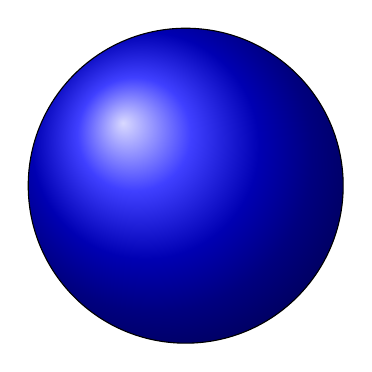
\begin{tikzpicture}
          \draw[shading = ball] (0, 0) circle (2);
    \end{tikzpicture}
\end{document}
    \caption[One ball]{One ball.}
\end{figure}

% Standalone with \includegraphics:
\begin{figure}[thbp]
    \centering
    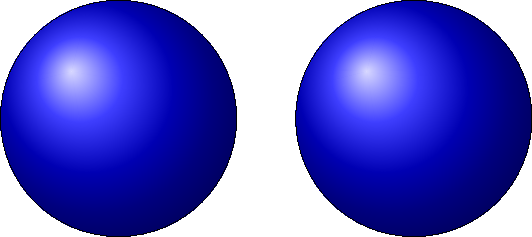
\includegraphics{balls}
    \caption[Two balls]{Two balls.}
\end{figure}

% Todonotes:
\begin{figure}[hbp]
    \centering
    \missingfigure{Three balls.}
    \caption[Three balls]{Three balls.}
\end{figure}

\kant[5-6] % Dummy text

% Booktabs:
\begin{table}[htbp]
    \centering
    \begin{tabular}{@{}ll@{}}
        \toprule
        \textbf{Correct}               & \textbf{Incorrect}      \\
        \midrule
        \( \varphi \colon X \to Y \)   & \( \varphi : X \to Y \) \\[0.5ex]
        \( \varphi(x) \coloneqq x^2 \) & \( \varphi(x) := x^2 \) \\
        \bottomrule
    \end{tabular}
    \caption[Colons]{Proper colon usage.}
\end{table}

\begin{table}[htbp]
    \centering
    \begin{tabular}{@{}ll@{}}
        \toprule
        \textbf{Correct}     & \textbf{Incorrect}         \\
        \midrule
        \( A \implies B \)   & \( A \Rightarrow B \)      \\
        \( A \impliedby B \) & \( A \Leftarrow B \)       \\
        \( A \iff B \)       & \( A \Leftrightarrow B \)  \\
        \bottomrule
    \end{tabular}
    \caption[Arrows]{Proper arrow usage.}
\end{table}

% Tablefootnote and multirow:
\begin{table}[htbp]
    \centering
    \begin{tabular}{@{}ll@{}}
        \toprule
        \textbf{Correct}
        & 
        \textbf{Incorrect}
        \\
        \midrule
        \( -1 \) 
        & 
        -1
        \\[0.3ex]
        1--10
        &
        1-10
        \\[0.3ex]
        Birch--Swinnerton-Dyer\tablefootnote{It is now easy to tell that Birch and Swinnerton-Dyer are two people.} conjecture
        &
        Birch-Swinnerton-Dyer conjecture
        \\[0.3ex]
        The ball \dash which is blue \dash is round.
        &
        \multirow{ 2}{*}{The ball - which is blue - is round.}
        \\[0.3ex]
        The ball---which is blue---is round. 
        &
        \\
        \bottomrule
    \end{tabular}
    \caption[Dashes]{Proper dash usage.}
\end{table}

\section{Outline}

The rest of the thesis is organised as follows:
\begin{description}
    \item[\cref{sec:second}]
    is second to none, with the notable exception of \cref{sec:intro}.
    The main tool introduced here is the employment of unintelligible sentences.
    
    \item[\cref{sec:third}]
    asserts the basic properties of being the third chapter of a thesis.
    This section reveals the shocking truth of filler content.
    
    \item[\cref{sec:fourth}]
    demonstrates how easily one can get to four chapters by simply using the \texttt{kantlipsum} package to generate dummy words.
    
    \item[\cref{sec:first-app}]
    features additional material for the specially interested.
    
    \item[\cref{sec:source}]
    consists of results best relegated to the back of the document,
    ensuring that nobody will ever read it.
\end{description}

    \part{The First Part}

    \chapter{The Second Chapter}
\label{sec:second}

\kant[7-11] % Dummy text

\begin{theorem}[{\cite[95]{AM69}}]
    \label{thm:dedekind}
    Let \( A \) be a Noetherian domain of dimension one. Then the following are equivalent:
    \begin{enumerate}
        \item \( A \) is integrally closed;
        \item Every primary ideal in \( A \) is a prime power;
        \item Every local ring \( A_\mathfrak{p} \) \( (\mathfrak{p} \neq 0) \) is a discrete valuation ring.
    \end{enumerate}
\end{theorem}
    \chapter{The Third Chapter}
\label{sec:third}
\kant[12-13] % Dummy text
\section{First Section}
\kant[14]    % Dummy text
\section{Second Section}
\kant[15]    % Dummy text
    \chapter{The Fourth Chapter}
\label{sec:fourth}
\kant[15-19] % Dummy text

    \appendix           % "Chapter" is renamed "Appendix"
    \appendixpage       % Similar to \part*{Appendices}, but appears in TOC

    \chapter{The First Appendix}
\label{sec:first-app}
\kant[20-21] % Dummy text
\section{First Section}
\kant[22]    % Dummy text
\section{Second Section}
\kant[23-24] % Dummy text
    \chapter{Source Code}
\label{sec:source}
\section{Implementation}
The \texttt{phduio} class is implemented in the following way:
\lstinputlisting[language = {[LaTeX]{TeX}}]{phduio.cls}

    \backmatter         % Folios in Arabic numerals, unnumbered chapters.

    \printbibliography

\end{document}